% !TeX encoding=utf8
% !TeX spellcheck = de_DE
% !TeX root = ../Diploma.tex

\chapter{Konzept des Clients}
In diesem Kapitel soll die Planung des Schachclients näher erläutert werden, welches als Grundbaustein für die Implementierung dienen soll. Dabei dient der erste Abschnitt zur Beschreibung der benötigten Anforderung, welche der Client erfüllen soll. Im zweiten Abschnitt sollen die einzelnen Ansichten, welche für eine bequeme Nutzerinteraktion benötigt werden, näher beschrieben. 

\section{Anforderungen}\label{sec:anforderungenClient}
Grundlegen soll der Client als Visualisierung des Servers dienen. Dafür soll dieser eine Verwaltung von Playern und Matches, inklusive dem anlegen neuer und dem bearbeiten, bereitstellen. Um anschließend auch Schach spielen zu können muss der Client dafür eine komfortable Möglichkeit, in Form eines Schachbrettes, bieten.\\
\\
Natürlich muss der Client außerdem mit dem Server kommunizieren können. Dafür muss dieser Requests senden und die empfangenen Response-Nachrichten verarbeiten können. Da der Server für manche Request spezielle Parameter benötigt, wie zum Beispiel einen String in der \gls{SAN}, muss der Client auch diese ermitteln können.\\
\\
Des weiteren soll der Client als \gls{SPA} erstellt werden und muss daher eine Möglichkeit zum Austauschen der einzelnen Ansichten, welche in dem \hyperref[sec:views]{Kapitel~\ref{sec:views}} genauer definiert werden, bieten.\\
\\
Für ein bequemes Spielerlebnis soll der Client ein gestartetes Match automatisch aktualisieren, sobald sich die Daten auf dem Server verändert haben. Dafür soll ein einfache Polling-Verfahren verwendet werden.\\
\\ 
Als letzte Grundanforderung soll eine innovative und benutzerfreundliche Bedienung der Anwendung sein, so das bis auf die Schachregeln keine weiteren Grundvoraussetzungen benötigt werden.

\section{Mock-Up-Entwicklung der benötigten Client-Ansichten}\label{sec:views}
In diesem Abschnitt sollen die im \hyperref[sec:anforderungenClient]{Kapitel~\ref{sec:anforderungenClient}} zuvor definierten Anforderungen konkretisiert und visuell aufbereitet werden. Die in diesem Kapitel erstellten Mock-Ups sollen die Implementierung vereinfachen bzw. beschleunigen.

\subsection{Startansicht}\label{sec:startView}
Diese Ansicht soll als Einstiegspunkte für Nutzer dienen, welche über diese die
Möglichkeit bekommen sollen zur Player-Ansicht bzw. zur Match-Ansicht zu wechseln. Die \hyperref[fig:startView]{Abbildung~\ref{fig:startView}} visualisiert dabei die zuvor definierten Anforderungen.
\begin{figure}[htb]
	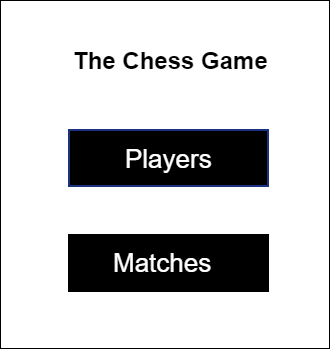
\includegraphics[width=0.9\textwidth]{images/start-view.png}
	\caption{Mock-Up: Startansicht des Clients}
	\label{fig:startView}
\end{figure}

\subsection{Player-Ansicht}\label{sec:playerView}
Inhalt dieser Ansicht soll die Möglichkeit zur Verwaltung von Playern sein. Dafür soll eine Tabelle mit allen angelegten Playern und ein Formular zum anlegen bzw. bearbeiten bereitstehen. Visuell unterstreicht die \hyperref[fig:playerView]{Abbildung~\ref{fig:playerView}} die definierten Anforderungen.
\begin{figure}[htb]
	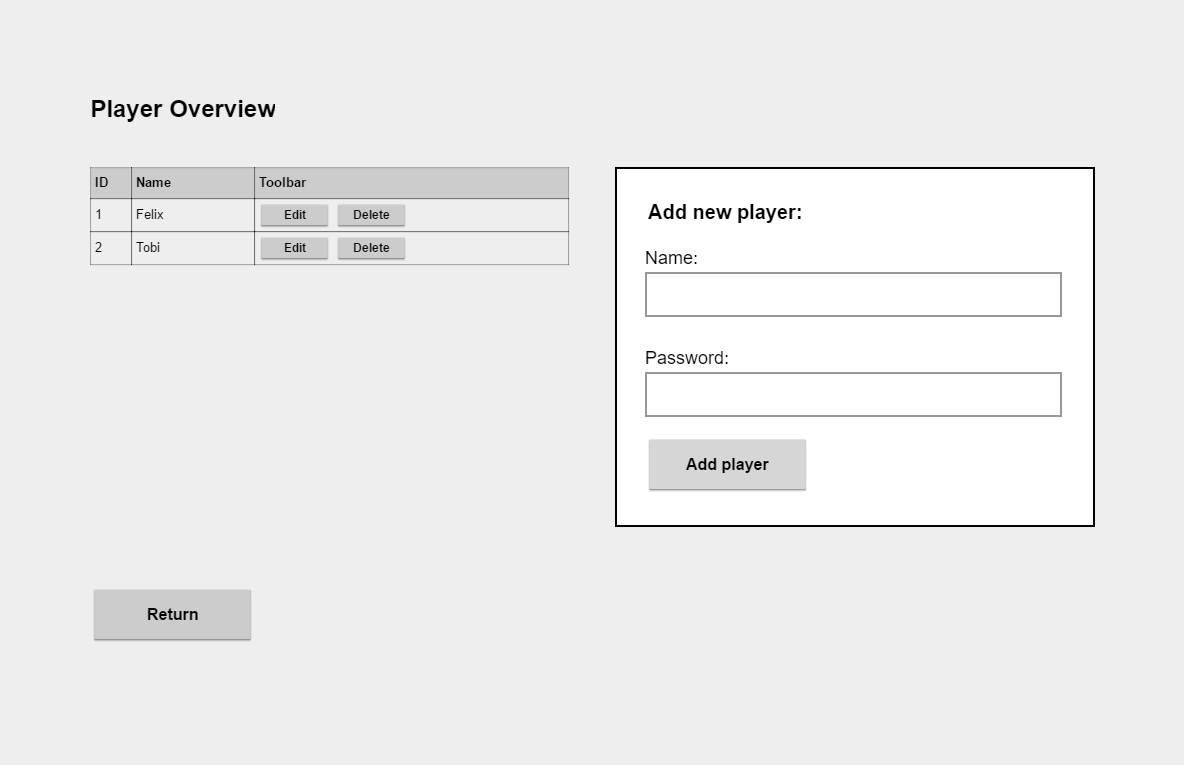
\includegraphics[width=0.9\textwidth]{images/player-view.png}
	\caption{Mock-Up: Player-Ansicht des Clients}
	\label{fig:playerView}
\end{figure}

\subsection{Match-Ansicht}\label{sec:matchView}
Mithilfe der Match-Ansicht soll die Verwaltung der Matches möglich sein. Hierfür soll wie bei der Player-Ansicht eine Tabelle mit angelegten Matches und ein Formular zum anlegen bereitstehen. Durch die \hyperref[fig:matchView]{Abbildung~\ref{fig:matchView}} werden die Anforderung grafisch dargestellt.
\begin{figure}[htb]
	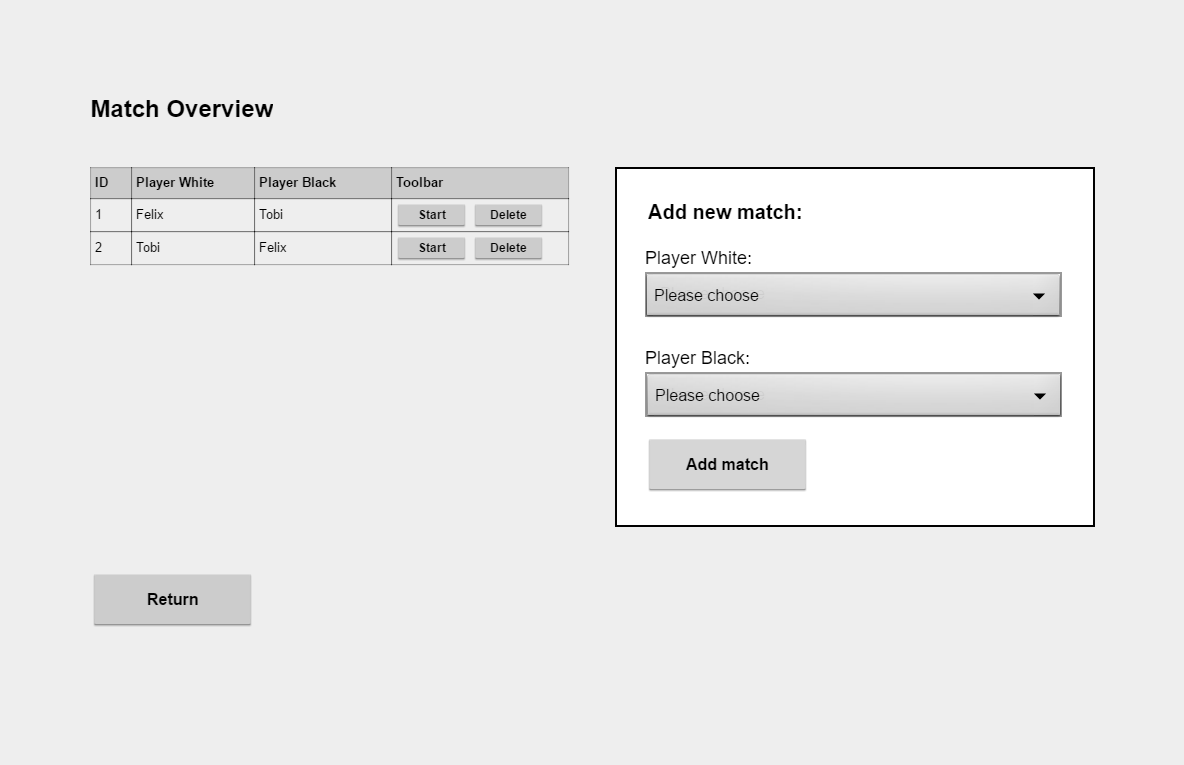
\includegraphics[width=0.9\textwidth]{images/match-view.png}
	\caption{Mock-Up: Match-Ansicht des Clients}
	\label{fig:matchView}
\end{figure}

\subsection{Ansicht eines gestarteten Matches}\label{sec:gameView}
Durch diese Ansicht soll die Möglichkeit zum Schach spielen bereitgestellt werden. Um spielen zu können wird in erster Linie ein Schachbrett benötigt, auf welchem die Figuren dargestellt werden. Mittels \enquote{Drag \& Drop} sollen dabei Spielfiguren bewegt und mittels \enquote{Mouseover} sollen möglichen Züge anzeigt werden können. Neben dem Schachbrett soll eine Reihe von Informationen bereitgestellt werden. Inhalt dieser sollen die geschmissenen Figuren, eine Liste aller Züge und ob sich ein Player im Schach befindet sein. Die \hyperref[fig:gameView]{Abbildung~\ref{fig:gameView}} zeigt die visuelle Darstellung der Anforderungen.
\begin{figure}[htb]
	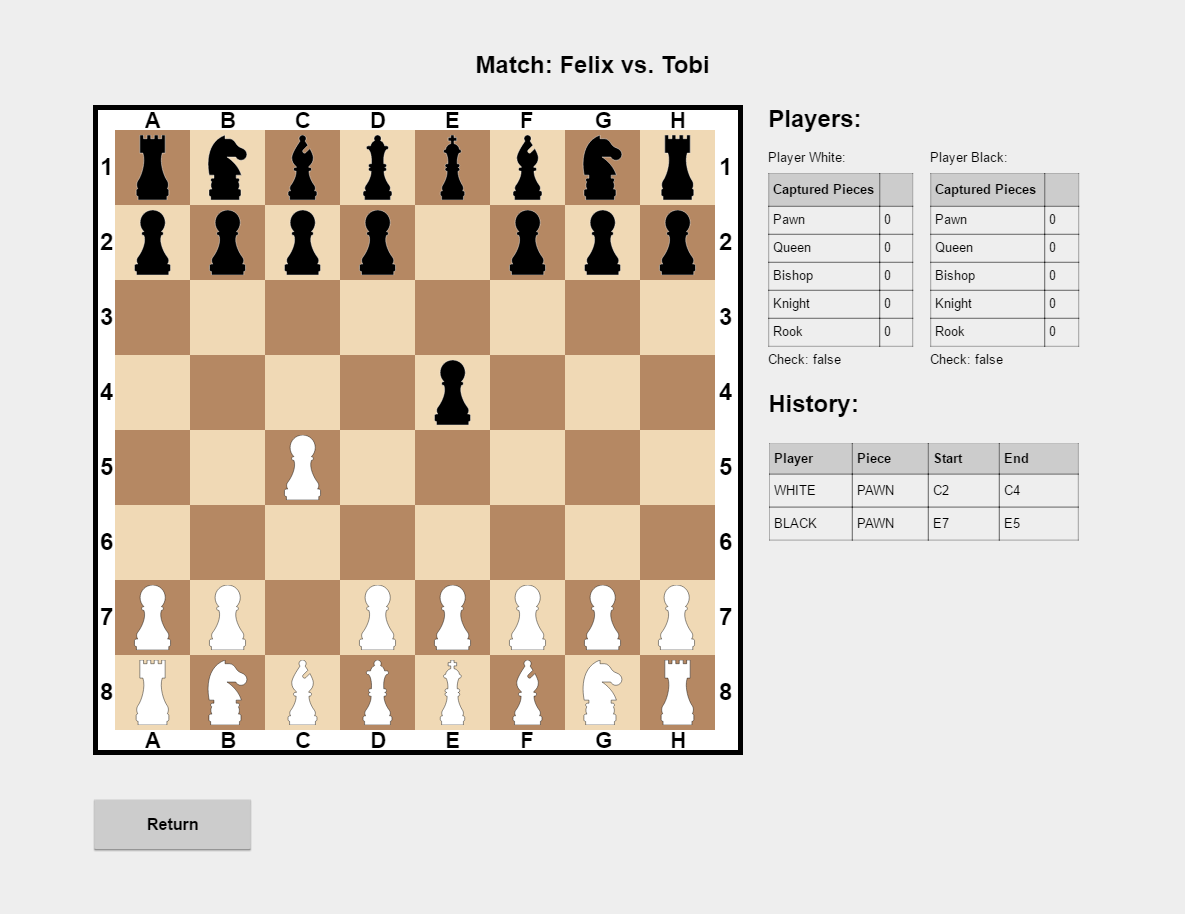
\includegraphics[width=0.9\textwidth]{images/game-view.png}
	\caption{Mock-Up: Ansicht eines gestarteten Matches}
	\label{fig:gameView}
\end{figure}


